\documentclass[hyperref={pdfpagelabels=false}]{beamer}
\usepackage{lmodern}
\usepackage{xcolor}
\usepackage{amsmath}
\usepackage{ragged2e} % para justificar
%\apptocmd{\frame}{}{\justifying}{} % Se quiser justificar todos os slides
\usepackage{hyperref}


\usepackage[options]{natbib}
\bibliographystyle{apalike}

\usepackage{tabularray}
\UseTblrLibrary{booktabs}

%\usetheme{CambridgeUS}
\usetheme{Berlin}
\usecolortheme{lily}

\definecolor{greenfriendly}{HTML}{164c64}
\definecolor{bondiblue}{rgb}{0.0, 0.58, 0.71}
\definecolor{VividCerulean}{HTML}{00AAEE}
\definecolor{myblue}{RGB}{33,84,157}

% citação abreviada como o título reduzido 
\title[The Hidden Cost of Bananas] { The Hidden Cost of Bananas:  \\ The Effects of Pesticides on Newborns’ Health  \\  \vspace{5mm} \large \textcolor{myblue}{Joan Calzada, Meritxell Gisbert, Bernard Moscoso} }



\author[Vinícius Hector and Natália Trigo]{ \normalsize Vinícius Hector \and Natália Trigo}
\date{March 26, 2024} 
\institute[]{ \textcolor{myblue}{ \href{https://www.journals.uchicago.edu/doi/abs/10.1086/725349?journalCode=jaere}{JAERE (2023) }}\\ \vspace{2mm} Environmental and Urban Economics \\ Professor: Sophie Mattes}
\begin{document}
	
	\begin{frame}
		\titlepage
	\end{frame} 
	
	
	\begin{frame}
		\frametitle{}
		\tableofcontents
	\end{frame} 
	
	
	\section{Motivation} 
	\begin{frame}
        \begin{itemize}
        \justifying
            \item Increasing demand for agricultural  productions, combined with land restrictions and changing weather has contribuited to the extensive use of agrochemicals
            \vspace{2mm}
            \item \textcolor{bondiblue}{Issue}:This use of chemicals has severe negative effects on the populations living close to the farms or working on them
            \vspace{2mm}
            \item But, still there are few studies analyzing the effects of enviromental pollution on health outcomes
            \vspace{2mm}
            \begin{enumerate}
                \item very few that leverage quasi-experimental variation to estimate the health effects of the use of pesticides in agriculture
            \end{enumerate}
            \vspace{2mm}
            \item \textcolor{bondiblue}{Goal of this paper}: examine the effects of pesticides used in banana plantations in Ecuardor on newborn's health outcomes
        \end{itemize}
 

        \end{frame}


        \begin{frame}{Why Ecuador?}
            \begin{itemize}
            \justifying
                \item Provides an excellent context for analysing the effects of pesticides use in agriculture
                \vspace{2mm}
                \item Ecuador is the world's fifth largest banana producer and the largest exporter
                \vspace{2mm}
                \item In the early 1970s, started to use aerial fumigations to treat fungal disease affecting banana fruit plants
                \vspace{2mm}
                \item \textcolor{bondiblue}{raised major concerns about their environmental and health implications}
            \end{itemize}
        \end{frame}

        \section{Empirical Strategy}
        \begin{frame}{Empirical Strategy}

        \begin{itemize}
        \justifying
            \item DiD approach that exploits the seasonal changes in the fumigation of banana plantations as an identification strategy
            \vspace{2mm}
            \item 4 newborn's health outcomes: weight at birth, gestational length, low birth weight, and preterm
            \vspace{2mm}
            \item Use of mother's address durirng pregancy and precise information on the perimeter of the plantations to compute measures of exposure to air pollution
            \begin{enumerate}
            \vspace{2mm}
                \item compute the mother's distance from the plantation and the area of fumigated plantations near their place of residence
            \end{enumerate}
        \end{itemize}
            
        \end{frame}

        \begin{frame}{}
        
        \begin{itemize}
        \justifying
            \item the newborns potentially most affected by pesticides were those born to mothers living within 150 meters of fumigated plantations
            \vspace{2mm}
            \item The paper use this result to construct a geographical exposure dummy variable (\textcolor{myblue}{\textbf{Banana Exposure}}) that defines the group of treated and control newborns
            \vspace{2mm}
            \item \textcolor{bondiblue}{Challenge}: households living close to the plantations present different characteristics from those living further way 
            %\textcolor{pink}{unobserved socioeconomic characteristics of households might affect both newborn's health outcomoes and the location of their residence}
           \vspace{2mm}
            \item \textcolor{bondiblue}{Approach}: exploits the seasonal changes in the intensity of fumigations. Fumigations are more intense during rainy season, which is when the fungus propagates more easily.
          
        \end{itemize}
            
        \end{frame}

        \begin{frame}{}
            \begin{itemize}
            \justifying
                \item They compute a seasonal exposure dummy (\textcolor{myblue}{\textbf{Intensive Fumigations}})
                \begin{enumerate}
                \justifying
                    \item create a grid of 5x5 km cells
                    \item the seasonal exposure variable takes the value 1 for newborns who during their gestation were for at least three months in a grid cell with more than four gallons of peticides per hectare.
                   \end{enumerate}
                  \item DiD strategy is based on the seasonality of the fumigations of the plantations surronding the mother's residence
                  \vspace{2mm}
                 \item DiD approach compares:
                 \begin{enumerate}
                 \justifying
                     \item  the difference between newborns born to mothers living in geographically exposed areas who were gestated during intensive and nonintensive fumigation seasons \\
                     \textcolor{red}{relative to}
                     \item the difference between newborns born to mothers living in geographically nonexposed areas who were gestated during the same two seasons
                 \end{enumerate}
            \end{itemize}
        \end{frame}

   \begin{frame}{}
       \begin{equation}
           Y_{ijmy} = \beta_{0} + \beta_{1}\text{Banana Exposure}_{ijmy} + \beta_{2}\text{Intensive Fumigations}_{ijmy} + \\ \theta \text{Banana Exposure}_{ijmy} \times \text{Intensive Fumigations}_{ijmy} + \\ \vspace{2mm} \delta X_{i} + \mu_{j} + \psi_{m} + \pi_{y} + \epsilon_{ijmy} 
       \end{equation}
       
       \vspace{4mm}


\hline


 \begin{equation}
           Y_{ijmy} = \beta_{0} + \beta_{1}\text{Banana Exposure}_{ijmy} + \sum_{z=1}^{3} \beta_{z} Z^{th}\text{Intensive Fumigations}_{ijmy} + \\  \sum_{z=1}^{3} \theta_{z} Z^{th}\text{Banana Exposure}_{ijmy} \times   Z^{th}\text{Intensive Fumigations}_{ijmy} + \\  \vspace{2mm} \delta X_{i} + \mu_{j} + \psi_{m} + \pi_{y} + \epsilon_{ijmy} 
       \end{equation}

       
   \end{frame}



        \begin{frame}{}

        \begin{itemize}
        \justifying
            \item $Y_{ijmy}$: birth outcomes of newborn $i$, in a grid cell $j$, month $m$ and year 
            \vspace{2mm}
            \item $\text{Banana Exposure}_{ijmy}$: is a dummy variable that takes the value 1 for newborns from mothers geographically exposed to pesticides
            \vspace{2mm}
            \item $\text{Intensive Fumigations}_{ijmy}$: is a dummy variable that takes the value 1 for newbornds that were affected by intensive fumigations for at least theree months during gestation
            \vspace{2mm}
            \item $Z^{th}\text{Intensive Fumigations}_{ijmy}$: is a dummy variable that takes the value 1 for the newbornds that were affected by intensive fumigations during the three months of the $Z^{th}$ gestation trimester.
            \vspace{2mm}
            \item $X$: vector of controls
        \end{itemize}
            
        \end{frame}
        

        \section{Data}

        \begin{frame}{Data}
        
\textbf{Newborn's health:}
        \begin{itemize}
        \justifying
        
            \item dataset from the National Register of Live Births for the period 2015-17  (information on the mother's residential addresses during pregancy)
            \item data set includes information on several observable characteristics of children and mothers
            \end{itemize}
    \textbf{Ecuador's banana plantations:}
            \begin{itemize}
                \item 2013 agricultural census
                \item 2016-18 register of aerial fumigations (geocoded data on the application of the pesticide)
            \end{itemize}
            
        \end{frame}

\begin{frame}{}

\begin{figure}[H]
    \centering
    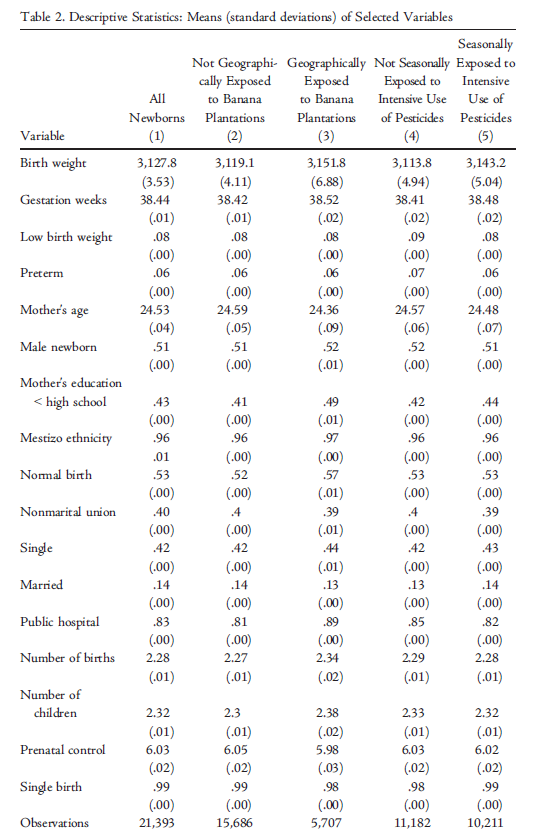
\includegraphics[width=6cm, height=7cm]{figures-paper/table2.png}
    \caption{Table 2 from Calzada, Gisbert, and Moscoso (2023)}
    \label{fig:enter-label}
\end{figure}
    
\end{frame}

\begin{frame}
\begin{figure}[H]
    \centering
    \includegraphics[width=6cm, height=7cm]{}
    \caption{Table 2 from Replication}
    \label{fig:enter-label}
\end{figure}
    
\end{frame}





   \begin{frame}{Preview of the results}
    \begin{itemize}
        \item pesticides have a statistically significant impact on newborns' birth weigth
        \item pesticides have a greater impact when intensive fumigations coincide with the first two trimesters of gestation
        \item exposure to pesticides reduces the number of gestations weeks and increases the odds of being born with low birth weight and of preterm delivery
    \end{itemize}


       
   \end{frame}

\section{Results}

\begin{frame}{Results}

\begin{figure}
    \centering
    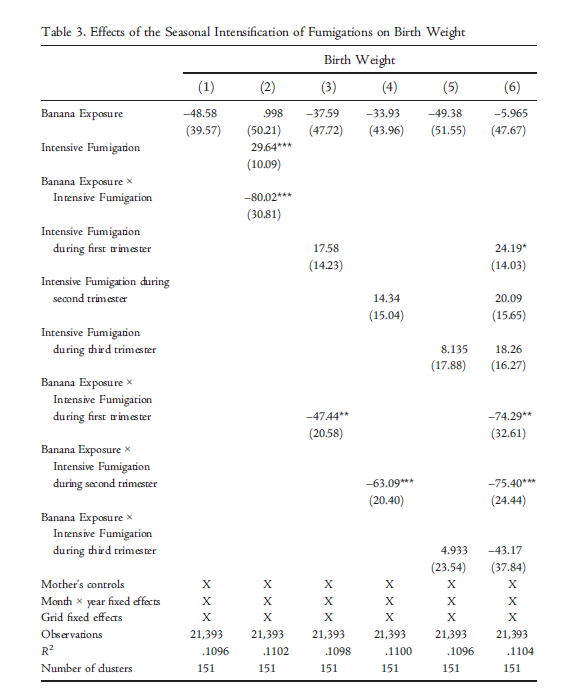
\includegraphics[width=6cm, height=6cm]{figures-paper/table3.png}
    \caption{Table 3 from Calzada, Gisbert, and Moscoso (2023)}
    \label{fig:enter-label}
\end{figure}
   
\end{frame}

 \begin{frame}{}

\begin{figure}
    \centering
    \includegraphics[width=8cm, height=8cm]{}
    \caption{Table 3 from  replication}
    \label{fig:enter-label}
\end{figure}

    
\end{frame}

 \begin{frame}{}

\begin{figure}
    \centering
    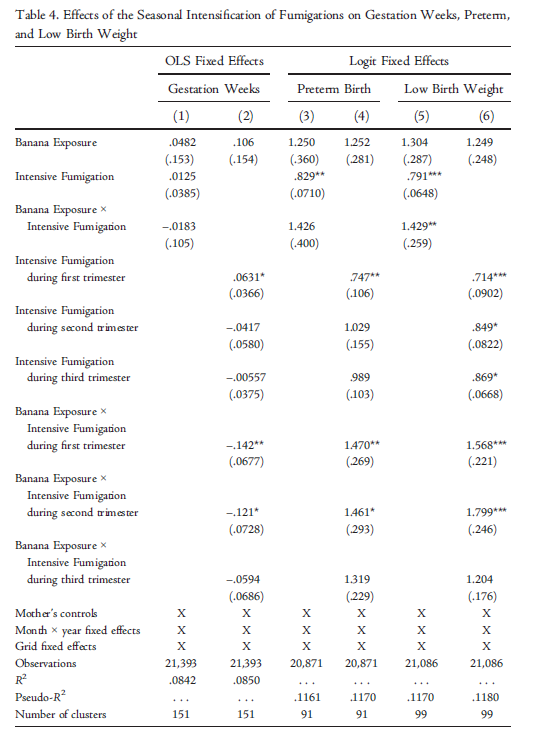
\includegraphics[scale=0.4]{figures-paper/table4.png}
    \caption{Table 4 from Calzada, Gisbert, and Moscoso (2023)}
    \label{fig:enter-label}
\end{figure}

    
\end{frame}


 \begin{frame}{}

\begin{figure}
    \centering
    \includegraphics[width=6cm, height=6cm]{}
    \caption{Table 4 from  replication}
    \label{fig:enter-label}
\end{figure}

    
\end{frame}

 \begin{frame}{}

\begin{figure}
    \centering
    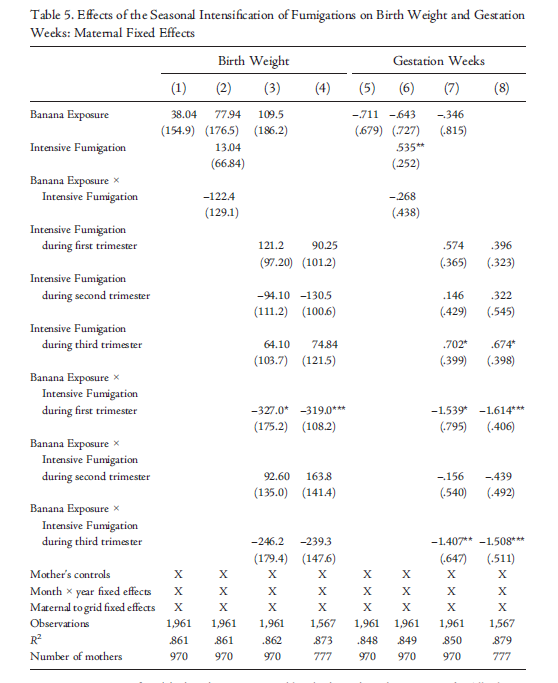
\includegraphics[scale=0.4]{figures-paper/table5.png}
    \caption{Table 5 from Calzada, Gisbert, and Moscoso (2023)}
    \label{fig:enter-label}
\end{figure}
   
\end{frame}

 \begin{frame}{}

\begin{figure}
    \centering
    \includegraphics[width=6cm, height=6cm]{}
    \caption{Table 5 from  replication}
    \label{fig:enter-label}
\end{figure}

    
\end{frame}


\end{document}







        \begin{comment}
            
	\begin{frame}
		\frametitle{References}
		%\printbibliography
		\bibliography{references.bib}
	\end{frame}
	\end{comment}
	
